\documentclass[10pt]{article}
\usepackage{graphicx}
\usepackage[margin=25mm]{geometry}
\linespread{1.3}

\title{Extensive Summary}
\author{Pedro Corrêa Pereira Vasco de Lacerda}

\begin{document}
\maketitle
Most neurons in the brain interact with each other by generating an action potential (AP), a fast, transient, and stereotypical fluctuation in the membrane potential of the cell, commonly referred to as a spike. The AP propagates along the neuron following a consistent trajectory from the soma (the neuron's body) through the axon to the synapse. 
The changes in membrane potential cause ions to flow in and out of the neuron and, consequently, cause a disturbance in the charge distribution in the extracellular medium, producing the Extracellular Action Potential (EAP). The EAP propagates outwards in the extracellular medium. \cite{kandel}

while intracellular action potentials AP are very stereotyped, the EAPs waveform show a large variability. Not only morphologic aspects of the neuron influence the characteristics of the EAP, but as the AP is propagated intracellularly there is a continuous generation of EAPs  down the axon. This leads a complex propagation of the EAP through the extracellular medium. \cite{gold2006origin}

To study the dynamics of neural activity, electrophysiology is still the most widely used, in particular, extracellular recording, which measures the voltage fluctuations that surround the electrodes, including the EAPs generated relatively close to the electrode.

In the last decades, extracellular electrophysiology has been done using probes with more and more electrodes, in particular large probes where the electrodes are closely positioned. This allows for sampling of the EAP in different positions in space, which produces a characteristic "foot print" on the probe, facilitating the identification the EAP.
 
The signal is acquired and then, usually offline, the data is processed and spike detection is performed, where researcher try to find when a spike took place. Then the detected spikes are assigned to one neuron, through a process called spike sorting.

Furthermore, since these new generation probes are larger, they are prone to sensing temporally overlapping spikes, which doesn't happen very often with tetrodes.

While many different methods for spike sorting have been proposed, no method is robust enough to be widely adopted by the experimental community.

To take advantages of the spatiotemporal characteristic of each EAP, Rossant et al. \cite{Rossant2016} proposed a method for spike detection that uses information about the geometry of the probe to define coherent regions were the EAP occured. This seem to be the best solution for dealing with the overlap of EAP above mentioned.

In \cite{Netoetal}, they perform paired recording with a juxtacellular pipette and new generation silicon probes with 32 and 128 electrodes. 

The dataset consists of twenty-three paired recording with a distance of less than 200 $\mu m$ between the targeted neuron and the closest extracellular electrode. These were acquired from twenty-three cells, from the cortex of several anesthetized rats.

With this dataset we have a precise determination of when one neuron was active. With this information it is possible to compute triggered averages allowing for the study of the propagation of the EAP.

Also, with this dataset it is possible to evaluate the performance and limitations of spike detection and spike sorting algorithms. In particular, in \cite{Rossant2016}, a method was developed that uses the information about the relative position of electrodes in a multi-electrode array in order to take advantage of the “neuron footprints”.

This signal from the extracellular probe doesn't usually have a high SNR. To get the waveform of the EAP on this probe we perform Juxta-Triggered Averages (JTAs), where windows of 4 ms centered on the juxta spikes are averaged so that the noise decreases and the waveform becomes clear.

During the course of this project I focused on 5 recordings where the 128-channels probe was used. These are summarized in Table \ref{tab:sum-recordings}.


\begin{table}[!h]
\centering
\begin{tabular}{ccccc}
\textbf{Recording ID} & \textbf{Short ID} & \textbf{Distance ($\mu m$)} & \textbf{P2P ($\mu V$)} & \textbf{Juxta spikes}\\ \hline
2015\_09\_09\_Pair7.0 & 997 & 136.2 $\pm$ 40 & 20.7 & 1082  \\ 
2015\_09\_04\_Pair5.0 & 945 & 96.1 $\pm$ 40 & 30.8 & 185  \\ 
2015\_09\_03\_Pair6.0 & 936 & 153.3 $\pm$  40 & 24.1 & 3329 \\ 
2015\_09\_03\_Pair9.0 & 939 & 11.5 $\pm$  40 & 416.3 & 5007  \\ 
2015\_08\_21\_Pair3.0 & 8213 & 132.8 $\pm$ 40 & 19.4  & 8117 \\ 
\end{tabular}
\caption{Information about the recordings used. The values on the "Recording ID" are conform the dataset provided by \cite{Netoetal}. For convenience, a Short ID will be used throughout this document. P2P stands for Peak-to-Peak Amplitude calculated as the $\max_i \left( \max_t \left( JTA_i \right) - \min_t \left( JTA_i \right)\right), i=0,\ldots , 127$. In the fifth column are the values of the depth in the cortex. In the last column are the number of spikes detected in the signal from the Juxtacellular pipette.}
\label{tab:sum-recordings}
\end{table}

We have some variability in this ensemble. 
The recording 939 was recorded very closed to the neuron and therefore has a very large P2P amplitude and lies above the noise; it also recorded many spikes. 
The recording 945 has a very low count of spikes and relatively low P2P amplitude. For this reason its JTA is not very well defined.
Despite its low P2P amplitude, the recording 8213 is the one with the most events, making its JTA reasonable.

%%%%%%%%%%%%%%%%%%%%%%%%%%%%%%%%%%%%%%%%%%%%%%%%%%%%%%%%%%%%%%%%%

First, I applied the SpikeDetekt using phy (a command-line implementation of SpikeDetekt and KustaKwik) from Rossant et al. to the five recording mentioned above.

SpikeDetekt requires the user to define many parameters prior to running: most significantly the  weak and strong thresholds. The authors report that the optimal values for these parameters are $\theta_w = 2 \sigma_{noise}$ and $\theta_s = 4.5 \sigma_{noise}$ where $\sigma_{noise}$ is the standard deviation of the noise for each channel which is estimated as the standard deviation estimator $s_{n-1}$ of a few time windows of the filtered signal spread across the whole recording.

%%%%%%%%%%%%%%%%%%%%%%%%%%%%%%%%%%%%%%%%%%%%%%%%%%%%%%%%%%%%%%%%%
%To analyze neural activity in the brain, scientists often look into the temporal correlation of the recorded signals.
%
%
%When performing this kind of analysis, spike signals are usually represented as a sequence of times when the neuron spiked or as a time series of 0's and 1's, if a sparse representation is preferred. These are called spike trains.
%
%This is usually done by means of calculating cross-correlograms. These are the graphical form of the cross-correlation between to signals, typically in the form of histograms.

%%%%%%%%%%%%%%%%%%%%%%%%%%%%%%%%%%%%%%%%%%


For each recording, phy (a command-line implementation of SpikeDetekt and KlustaKwik) was run with the following parameters:
The data was filtered with a forwards-backwards Butterworth filter of order 3 with cutoff frequency set to 500Hz. The noise standard deviation was evaluated in 50 excerpts of 1 second each. The weak threshold was $\theta_w = 2 \sigma_{noise}$ and the strong threshold was $\theta_s = 4.5 \sigma_{noise}$.

The results are presented in table \ref{tab:results-from-phy}.

\begin{table}[!h]

\begin{center}
\begin{tabular}{ccccc}
Recording ID & \# detected Spikes & $\sigma_{noise}$ ($\mu V$) & $\theta_W$ ($\mu V$) & $\theta_S$ ($\mu V$) \\ \hline
8213 & 148762 &  12.95 & 25.91 & 58.30 \\ 
936 & 323629 & 10.76 & 21.52 & 48.43 \\ 
939 & 265476 & 10.51 & 21.02 & 47.29 \\ 
945 & 126234 & 10.92 & 21.84 & 49.14 \\ 
997 & 156932 & 11.47 & 22.93 & 51.60 \\ 
\end{tabular}
\end{center}
\caption{Summary of the output from phy. In this table are the values of the estimated standard deviations of the noise, and the calculated weak and strong thresholds for each recording. These values were converted into $\mu V$.}
\label{tab:results-from-phy}
\end{table}


In Fig. \ref{fig:CC} are the whole-probe cross-correlograms for the recordings, where for each detected spike, all electrodes whose corresponding mask value was non-zero were used.

\begin{figure}[!h]
	\centering
	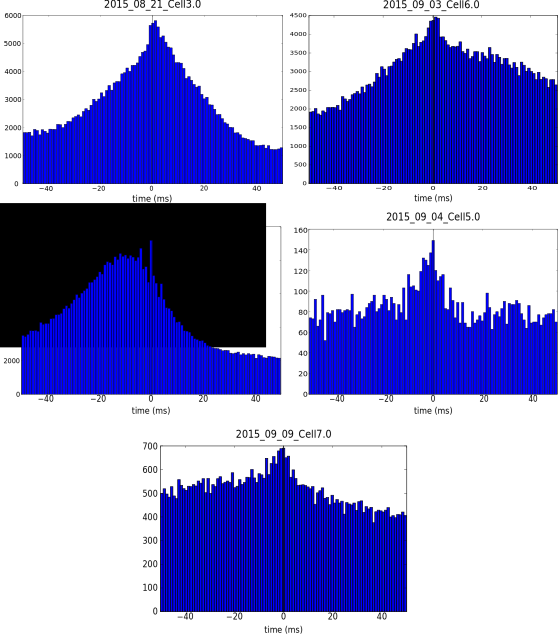
\includegraphics[width=0.8\linewidth]{CC.pdf}
	\caption{Cross-Correlograms for all the recordings. The size of the bins in the histograms is 1 ms and the value for the lag is 50ms.
}
\label{fig:CC}
\end{figure}


On Fig \ref{fig:CC}, all cross-correlograms present a somewhat coherent distribution. This means that for every value $\tau$ in the considered interval, there exists some temporal correlation between the juxta neuron and the activity of the rest of the neurons in the recorded volume. This is to be expected. According to Ruiz-Mejias et al., the use of ketamine as anesthesia in rats provokes the synchronization in the population activity in many cortical areas, including the motor cortex. This gives rise to "up" and "down" states, where most neurons in the population are firing or silent, respectively. In addition, they report that the frequency of oscillation of these states is, on average, 0.97Hz, which is close to the firing rates observed in the juxtacellular recordings from \cite{Netoetal}. 

Only on the cross-correlogram corresponding to the recording 939 can we see a distinct peak when $\tau=0 ms$, on top of the correlation with the background activity. This means that phy managed to find juxta neuron.

On the rest of the cross-correlograms in Fig \ref{fig:CC}, the peak around the central bin is never very clear. In fact, in the case of the recordings 8213 and 936, the peak is even shifted to $\tau=1 ms$. This could justify a more careful examination setting the size of the bin used in the histograms to a smaller value.

To calculate the number of events corresponding to the juxta, it is necessary to remove the counts from the correlation with the background activity. To estimate this value, the average of the counts in the bin neighboring bins ($\tau = -1ms$ and $\tau = 1 ms$) was computed and subtracted to the counts in the central bin. The results are in table \ref{tab:CCcorrection}.

\begin{table}[!h]
\begin{center}
\begin{tabular}{p{1.5cm}|c|c|c|p{1.3cm}|c|r}

\multicolumn{ 1}{p{1.5cm}|}{Recording ID} & \multicolumn{ 3}{c|}{Bin Counts} &  \multicolumn{ 1}{p{1.3cm}|}{Corrected Counts} & \multicolumn{ 1}{c|}{\#juxtaSpikes} & \multicolumn{ 1}{c}{Accuracy} \\ 
\multicolumn{ 1}{c|}{} & $\tau=0$ & $\tau=-1$ & $\tau=1$ & \multicolumn{ 1}{c|}{} & \multicolumn{ 1}{p{1.3cm}|}{} & \multicolumn{ 1}{l}{} \\ \hline
8213 & 5725 & 5642 & 5810 & -1 & 7760 & -0.01\% \\ 
936 & 4377 & 4357 & 4465 & -34 & 3329 & -1.02\% \\ 
939 & 9202 & 6701 & 7092 & 2305.5 & 4947 & 46.60\% \\ 
945 & 144 & 137 & 120 & 15.5 & 185 & 8.38\% \\ 
997 & 691 & 689 & 650 & 21.5 & 1082 & 1.99\% \\ 
\end{tabular}
\end{center}
\caption{Correction of the cross-correlograms central peak.}
\label{tab:CCcorrection}
\end{table}

Even in the recording 939 the detection rate is fairly low, considering it has a very large P2P amplitude.
In the other cases, phy yields a detection accuracy close to zero. This is not surprising considering the algorithm used by phy. The maximum P2P amplitude of JTAs of these case lies between lies between 19.4$\mu V$ and 30.8$\mu V$ and the strong threshold is always larger than 48.43 $\mu V$. Since it is required that at least one sample in a connected component be larger than the strong threshold these spikes are never detected. Two possible explanations exist for this number of detected events. First, the neuron may have spiked simultaneously to a large noise fluctuation causing it to be detected. Secondly, the connected components of these spikes could have been connected with the connected component of other spike which exceeded the strong threshold. This would result in the detection one single spike where the computed spike time was closer to the corresponding juxta spike time and therefore contributed to the central bin in the cross-correlograms.

%%%%%%%%%%%%%%%%%%%%%%%%%%%%%%%%%%%%%%%%%%%%%%%%%%%%%%%%%%%%%%%

These paired recordings can be seen as labeled datasets where each portion of the extracellular recording is assigned a classification regarding whether or not it contains an EAP from the neuron the juxtacellular probe was recording from. This seems a suitable setup for uses of machine learning techniques, in particular, supervised deep  learning.

A Deep Neural Network (DNN) is a artificial neural network with at least three layers. This way one can define a model in such a way that each layer has a different representation of the input layer. Each layer is a more abstract representation than the layer that preceeds it. This allows very complex and human-like computation.

In this part of the project we defined the basic model of DNN to be utilized as a fully-connected feed-forward DNN with:
\begin{itemize}
\item 5 layers
\item First layer with 12700, second third and fourth layer with 200 neurons and the fifth layer with one neuron
\item ReLU as activation function for hidden units and Sigmoid for the output neuron
\item Adagard as the training algorithm
\item Cross-entropy for loss function
\item L1-Regularizer along with dropout with probability parameter set to 0.2
\end{itemize}

Using the recording 939, a study on the performance of the DNN was made. The optimal parameters were found to be:
\begin{itemize}
\item The Learning Rate $\eta = 0.001$
\item The weight decay $\lambda = 0.01$
\item The initialization Method was LeCun uniform
\end{itemize}

These optimal hyperparameters and configurations discussed were used in the training of the DNN with each the datasets. The performance results are in Fig. \ref{fig:study-cells}

\begin{figure}[!Ht]
	\centering
	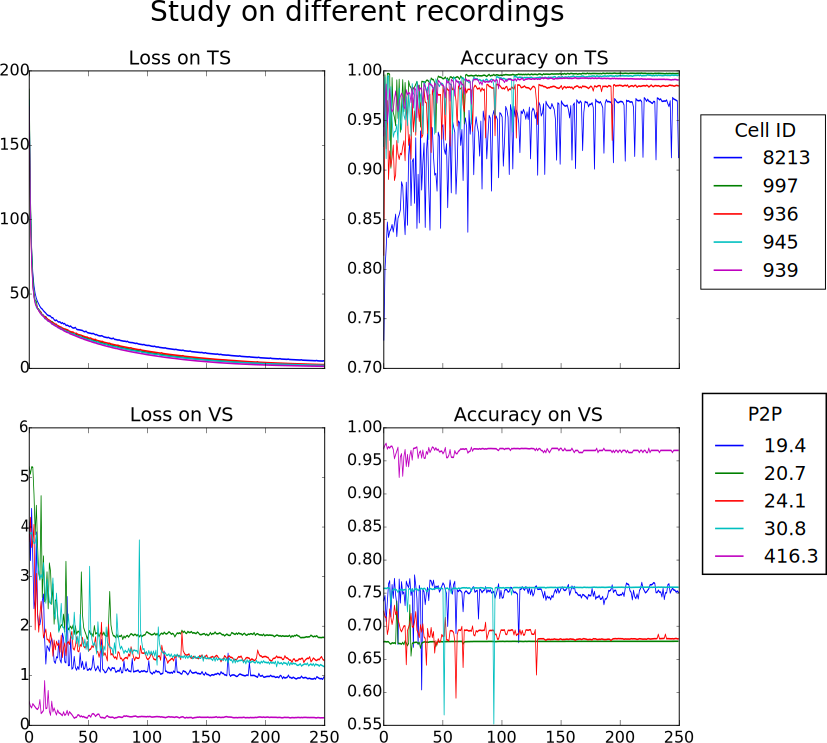
\includegraphics[width=0.8\linewidth]{study_on_different_cells_v2.pdf}
	\caption{Study on Different Recordings. Loss function and accuracies in the training set and in the validation set.The learning rate was $\eta = 0.001$, the weight decay was fixed at $\lambda = 0.01$, and the initialization method was LeCun Uniform. On the legend on the top is the Cell ID and on the legend on the bottom are the P2P amplitude.
}
\label{fig:study-cells}
\end{figure}

Looking at the accuracy on the training set, one can that the accuracy always gets better along the epochs. However on the validation set, the accuracies seem to converge fairly quickly.
The figures present three different situations. On the case of the recording 939, an accuracy of around 97\% is achieved. Two cells converged to approximately 76\% and other two converged to approximately 68\%. 

\bibliographystyle{plain}
\bibliography{02.biblio}
\end{document}